\documentclass[9pt,twocolumn,twoside,lineno]{pnas-new}
% Use the lineno option to display guide line numbers if required.

\templatetype{pnasresearcharticle} % Choose template
% {pnasresearcharticle} = Template for a two-column research article
% {pnasmathematics} %= Template for a one-column mathematics article
% {pnasinvited} %= Template for a PNAS invited submission

% Math
\def\P{\mathbb{P}}
\def\cor{\mathrm{cor}}
\def\Quantile{\mathrm{Quantile}}
\def\logit{\mathrm{logit}}
\def\dist{\mathrm{dist}}
\def\WIS{\mathrm{WIS}}
\def\AUC{\mathrm{AUC}}
\newcommand{\indicator}[1]{\mathbf{1}\left(#1\right)}

% Figures and tables
\usepackage{xurl}
\usepackage{microtype}
\usepackage{booktabs}
\usepackage{caption}
\usepackage{subcaption}
\usepackage{xcolor}
\newcommand{\attn}[1]{\textcolor{red}{[ATTN: #1]}}

\makeatletter 
\renewcommand\@biblabel[1]{#1} 
\makeatother

% indicators
\newcommand{\chngcli}{CHNG-CLI}
\newcommand{\chngcov}{CHNG-COVID}
\newcommand{\dv}{DV-CLI}
\newcommand{\ar}{AR}
\newcommand{\fb}{CTIS-CLI-in-community}
\newcommand{\gs}{Google-AA}


\title{An Open Repository of Real-Time COVID-19 Indicators}

% Use letters for affiliations, numbers to show equal authorship (if applicable) and to indicate the corresponding author
\author[a,c,1]{Author One}
\author[b,1,2]{Author Two}
\author[a]{Author Three}

\affil[a]{Affiliation One}
\affil[b]{Affiliation Two}
\affil[c]{Affiliation Three}

% Please give the surname of the lead author for the running footer
\leadauthor{Lead author last name}

% Please add a significance statement to explain the relevance of your work
\significancestatement{To study the COVID-19 pandemic, its effects on society,
  and measures for reducing its spread, researchers need detailed data on the
  course of the pandemic. Standard public health data streams suffer
  inconsistent reporting and frequent, unexpected revisions. They also miss
  other aspects of a population's behavior, worthy of consideration. We
  present an open database of COVID signals in the United States, measured at
  the county level and updated daily. These include traditionally reported COVID
  cases and deaths, and many others: signals based on measures of mobility,
  social distancing, internet search trends, self-reported symptoms, and
  patterns COVID-related activity in de-identified medical insurance claims. The
  database provides all signals in a common, easy-to-use format, empowering both
  public health research and operational decision-making.
}

% Please include corresponding author, author contribution and author declaration information
\authorcontributions{Please provide details of author contributions here.}
\authordeclaration{Please declare any competing interests here.}
\equalauthors{\textsuperscript{1}A.O.(Author One) contributed equally to this work with A.T. (Author Two) (remove if not applicable).}
\correspondingauthor{\textsuperscript{2}To whom correspondence should be addressed. E-mail: author.two\@email.com}

% At least three keywords are required at submission. Please provide three to five keywords, separated by the pipe symbol.
\keywords{open data $|$ COVID-19 $|$ digital surveillance $|$ medical insurance
  claims $|$ internet surveys $|$ search trends $|$ mobility patterns}

\begin{abstract}
  Please provide an abstract of no more than 250 words in a single paragraph.
  Abstracts should explain to the general reader the major contributions of the
  article. References in the abstract must be cited in full within the abstract
  itself and cited in the text.
\end{abstract}

\dates{This manuscript was compiled on \today}
\doi{\url{www.pnas.org/cgi/doi/10.1073/pnas.XXXXXXXXXX}}

\begin{document}

\maketitle
\thispagestyle{firststyle}
\ifthenelse{\boolean{shortarticle}}{\ifthenelse{\boolean{singlecolumn}}{\abscontentformatted}{\abscontent}}{}

\dropcap{P}ublic health decision makers, healthcare providers, epidemiological 
researchers, employers, institutions, and the general public benefit from
promptly and readily accessible data regarding COVID-19 activity levels,
countermeasures, and pandemic impact.  Real-time indicators of COVID-19 
activity levels, such as statistics on cases, deaths, test positivity, and
hospitalizations, enable reports and interactive dashboard applications for
situational awareness \cite{Dong:2020, NYTimes, USAFacts}, and are essential for
most analyses of the pandemic.  These data are available for locations across
the United States from a number of official sources and independent aggregators
in varied and inconsistent formats.  Different data types and sources vary in
timeliness, based on when measured events occur in the progression of the
disease, testing capabilities, the reporting pipeline, and their publication
schedules.

Additional, auxiliary data sources can improve on the timeliness, scope, and
utility of the ``topline'' indicators (cases, test positivity, hospitalizations,
deaths) coming from the public health reporting system. For example, in the
context of other infectious diseases: syndromic surveillance in ambulatory
clinics and emergency rooms improves the accuracy of outbreak detection for
emerging pathogens such as H1N1 \cite{Kass-Hout:2012}; and digital surveillance
(based on, e.g., search and social media trends) enable more accurate
``nowcasts'' and forecasts of traditional disease surveillance streams such as
the CDC's ILINet \cite{Santillana:2015, Farrow:2016}, as do publication formats
providing access to historical versions of a data set \cite{Brooks:2018,
  Brooks:2020}. Numerous other examples exist spanning a wide variety of data
platforms and diseases \cite{Browstein:2009, Kass-Hout:2011, Salathe:2012,
  Kass-Hout:2013}. During the COVID-19 pandemic, digital data streams have
permitted faster prediction of case increases \cite{Ahmad:2020, Kogan:2021},
while enabling analyses of the impact of public health policies on public
behavior, the economy, and disease spread \cite{Bonaccorsi:2020, Nouvellet:2021,
  Adjodah:2021, Jewell:2021}.

The Delphi Group works with partner organizations and public data sets to build
a massive database of indicators tracking COVID-19 activity and other relevant
phenomena in the United States, which has been publicly available and
continuously updated since April 2020. Alongside public data on reported cases
and deaths, this database includes several unique data streams, including
indicators extracted from de-identified medical claims data, antigen test
results from a major testing manufacturer, large-scale public surveys that
measure symptoms and public behavior, and indicators based on particular Google
search queries. (We use the terms ``indicator'' and ``signal'' interchangeably.)
We make aggregate signals publicly available, generally at the county level, via
the COVIDcast API \cite{CovidcastAPI}. We store and provide access to all
previous (historical) versions of the signals, a key feature that exposes the
effects of data revisions.  Lastly, we provide R \cite{CovidcastR} and Python
\cite{CovidcastPy} packages to facilitate interaction with the API, and an
online dashboard to visualize the data \cite{CovidcastViz}. 

In a companion paper, we analyze the utility provided by a core set of the
indicators in COVID-19 forecasting and hotspot prediction models.  In another
companion paper, we elaborate on our research group's (Delphi's) large-scale
public surveys, run in partnership with Facebook and available in aggregate form
in the COVIDcast API.

\section{Methods}

\subsection{Data Collection}

We receive data daily from healthcare partners, technology companies, and from
surveys conducted daily by Delphi in partnership with Facebook. These data
sources provide information not available from standard public health reporting
or other common sources, such as:

\paragraph{Health Insurance Claims} Based on de-identified medical insurance 
claims from Change Healthcare and other health system partners, we release
indicators on the estimated percentage of covered outpatient visits and
hospitalizations that involved COVID diagnoses or symptoms.

\paragraph{Internet-Based Surveys} Conducted in partnership with Facebook,
Delphi's COVID Trends and Impact Survey receives an average of 50,000 responses
daily, and has received over 20 million responses since April 2020
\cite{DelphiSurvey, Kreuter:2020}. From the surveys, we construct indicators on
symptoms, social distancing, vaccination, and other attitudes and behaviors
related to COVID.  

\paragraph{COVID Antigen Tests} Based on data from Quidel, a manufacturer of
COVID antigen tests in the United States, we calculate and release
(Quidel-specific) test volumes and positivity rates.  

\paragraph{Search Trends} Based on Google's COVID-19 Search Trends data set
\cite{GoogleSymptoms}, we provide indicators reflecting COVID-related search  
activity.

\paragraph{Mobility Data} SafeGraph, a company that collects geospatial data
from smartphone apps, calculates COVID-related mobility signals
\cite{SafeGraphSocial, SafeGraphPatterns} and makes it available to researchers 
under a data use agreement; we aggregate (some of) these signals to the county
level and make them publicly available.     

\medskip
We also scrape data accessible from other public sources, such as cases and
deaths data aggregated from public reporting by JHU CSSE \cite{Dong:2020} and by
USAFacts \cite{USAFacts}, so that we can track revisions and updates to this data
(see Section~\ref{subsec:revision_tracking}).

Altogether, we collect 110 signals from 12 distinct sources, aggregate and
process them, and provide them in a common format for public access. This
unifies both unique (not available anywhere else) and standard COVID data
streams into a single common format, enabling efficient comparison and modeling.
A summary of the data sources and signals in the API is in
Table~\ref{tab:sources_signals}, and detailed documentation is available at 
\url{https://cmu-delphi.github.io/delphi-epidata/api/covidcast_signals.html}.

\begin{table*}[t]
\centering
\caption{Data sources available in Delphi's COVIDcast API \cite{CovidcastAPI},
  as of date of publication. The first group of data sources are produced by
  Delphi from data not otherwise available publicly (or only available in
  limited form); the second group is mirrored from public sources.}
\begin{tabular}{>{\raggedright}p{1.2in} p{4.0in} l >{\raggedright\arraybackslash}p{0.5in}}
  \toprule
  \textbf{Data source} & \textbf{Signals available} & \textbf{First date} &
\textbf{Resolution} \\\midrule
  % Exclusive data
  Change Healthcare & Percentage of outpatient visits with COVID diagnostic
codes or codes indicating COVID-like symptoms. Based on de-identified claims
data processed by Change Healthcare. & 2020-02-01 & County$^*$ \\
  Doctor Visits & Percentage of outpatient visits primarily about COVID-like
symptoms, based on de-identified claims data provided by health system
partners. & 2020-02-01 & County$^*$ \\
  Hospital Admissions & Percentage of new hospital admissions with COVID
diagnostic codes, based on de-identified claims data provided by health system
partners. & 2020-02-01 & County$^{**}$\\
  Quidel & Test positivity rates for COVID-19 antigen tests produced by
Quidel. & 2020-05-26 & County$^{**}$ \\
  SafeGraph & Mobility metrics, such as time away from home or visits to bars 
and restaurants, based on cell phone mobility data collected by SafeGraph
\cite{SafeGraphSocial, SafeGraphPatterns}. & 2019-01-01 & County \\
  COVID Trends and Impact Survey & COVID symptoms, social distancing 
behaviors, mental health, economic impact, behavior (e.g., mask-wearing,
vaccination attitudes), and COVID testing signals based on daily surveys
conducted nationally by Delphi through Facebook \cite{DelphiSurvey,
Kreuter:2020}. & 2020-04-06 & County$^{**}$ \\
  \midrule
  % Mirrored data from other sources
  Health \& Human Services & Counts of hospital admissions due to confirmed or 
suspected COVID-19, as reported by the Department of Health \& Human Services. &
2019-12-31 & State \\
  COVID Act Now & COVID-19 testing results, such as positivity rate and number
of tests, compiled by COVID Act Now from CDC reporting. & 2020-03-02 &
County$^*$ \\
  Google Symptoms & Trends in Google search volume for terms related to
anosmia and ageusia (loss of smell or taste), which correlate with COVID
activity, based on data shared by Google \cite{GoogleSymptoms}. & 2020-02-13 &
County$^{***}$ \\
  Cases and Deaths & Confirmed COVID-19 cases and deaths, compiled by JHU CSSE 
\cite{Dong:2020} and by USAFacts \cite{USAFacts}. & 2020-01-22 & County \\
    NCHS Mortality & Weekly totals of deaths broken down by cause, such as
COVID, flu, or pneumonia, compiled by the National Center for Health Statistics
\cite{NCHS}. & 2020-01-26 & State \\
  \bottomrule
\end{tabular}
\addtabletext{$^*$Available at $>60$\% of counties; $^{**}$available at
  20--60\% of counties; $^{***}$available at $<20$\% of counties.  For some
  signals, location availability varies over time, e.g., due to variable
  reporting volume.}
\label{tab:sources_signals}
\end{table*}

\subsection{Signal Processing}

Because each data source reports data in different formats, we must convert each
source to a common format. In this format, each record represents an observation
of one quantity at one time point in one location. Locations are coded
consistently using standard identifiers such as FIPS codes; the sample size and
standard error for each observation is also reported when applicable. Each
signal is reported at the finest geographic resolution its source supports (such
as county or state) and also aggregated to metropolitan statistical areas,
Health and Human Services regions, and hospital referral regions. National
averages are also provided. Crucially, each record is tagged with an
\textit{issue date} referring to when the value was first issued, as described 
below. This allows tracking of revisions made to individual observations, as
each revision is tagged with its own issue date.  

When appropriate, additional post-processing (often nontrivial) is applied to
the data. For example, data on visits to doctor's offices is subject to strong
day-of-week effects, and so regression is used to adjust for these
effects. Other indicators are available in raw versions and versions smoothed 
with a 7-day trailing average. All processing is done using open-source code 
written primarily in Python and R, and available publicly at
\url{https://github.com/cmu-delphi/covidcast-indicators/}.

\subsection{Revision Tracking}
\label{subsec:revision_tracking}

Many data sources that are useful for epidemic tracking are subject to revision
after their initial publication. For example, aggregated medical claims data may
be initially published after several days, but additional claims and corrections
may take days to weeks to be discovered, processed, and aggregated. Medical
testing data are also often subject to backlogs and reporting delays, and
estimates for any particular date are revised over time as errors are found or
additional data becomes available. This revision process is generally referred
to as \textit{backfill}.

For this reason, the COVIDcast API annotates every observation with two dates:
the \textit{time value}, the date the underlying events (such as tests or
doctor's visits) occurred, and the \textit{issue date} when Delphi aggregated
and reported the data for that time value. Importantly, there can be multiple
observations for a single time value with different issue dates, for example if
data is revised or claims records arrive late. Delphi tracks revisions to all
data sources we ingest, including external data sources (such as sources
tracking cases and deaths). Many external sources do not keep a public or
conveniently accessible record of revisions of their data.

For many purposes it is sufficient to use the most recently issued observation
at any a given time value, and the COVIDcast API returns the most recent issue
as its default. However, for some applications it is crucial to know what was
known \textit{as of} a specific date. For example, an epidemic forecasting model
will be called upon to make its forecasts based on preliminary data about recent
trends, so when it is trained using historical data, it should be trained using
the initial versions of that data, not updates that would have been received
later. Moreover, these revision records allow models to be modified to account
for noise and bias in early data versions, or to exclude data that is too new to
be considered stable, and to ``rewind'' time and simulate how these revised
models would have performed using only the versions of data available \textit{as
of} those times.

Research on data revisions in the context of influenza-like illness has shown
that backfill can significantly alter forecast performance \cite{Brooks:2018,
  Reich:2019}, and that careful training on preliminary data can reduce this
influence \cite{Brooks:2020}. We also investigate this in our companion paper on
forecasting, where we observe that training and validating models on finalized 
data yields overly optimistic estimates of true test-time performance.

% TODO: Cite this? https://arxiv.org/abs/2106.04420

\subsection{Public API}

The data described above is publicly available through the Delphi COVIDcast API
\cite{CovidcastAPI}.  By making HTTP requests specifying the data source,
signal, geographic level, and time period desired, users can receive data in
JSON or CSV form. For added convenience, we have written \texttt{covidcast} R
\cite{CovidcastR} and Python \cite{CovidcastPy} packages with functions to
request data, format it as a data frame, plot and map it, and combine it with
data from other sources.

The R and Python package software is public and open-source, at
\url{https://github.com/cmu-delphi/covidcast/}.  The API server software is
itself also public and open-source, at
\url{https://github.com/cmu-delphi/delphi-epidata/}.  Lastly, most data sources 
are provided under the Creative Commons Attribution license, and a small number
have additional restrictions imposed by the data source; see
\url{https://cmu-delphi.github.io/delphi-epidata/api/covidcast_licensing.html}.

\subsection{Interactive Visualization}

Since April 2020, Delphi has been maintaining and continually improving various
online visualization tools for the COVIDcast indicators \cite{CovidcastViz}.
These tools fetch data directly from the API, and allow for exploration of both 
temporal (e.g., time series graphs) and spatial (e.g., choropleth maps) trends
in the signals, as well as many other aspects, such as correlations, anomalies,
and backfill.  There is also a dedicated dashboard for exploring results from
the COVID Trends and Impact Survey.   

\subsection{COVID Forecasting} 

Since July 2020, Delphi has been regularly submitting short-term forecasts of
COVID-19 case and death incidence, at the state and county levels, to the
COVID-19 Forecast Hub \cite{ForecastHub}, under the name ``CMU-TimeSeries''.  
The process of building, training, and deploying our forecasting models
leverages much of the infrastructure described in this paper (such as the
COVIDcast API's \textit{as of} feature), and some of our forecasting systems
rely on auxiliary indicators (such as survey-based and claims-based COVID-like 
illness signals, described below, which we have used in case forecasting).  

\section{Results}

The indicators that are available in the COVIDcast API have been used in
dashboards produced by COVID Act Now \cite{CovidActNow}, COVID Exit Strategy
\cite{CovidExitStrategy}, and others; to inform the Delphi, DeepCOVID
\cite{Rodriguez:2021}, and the Institute for Health Metrics and Evaluation
(IHME) \cite{IHMEProj} COVID forecasting models; in various federal and state
government reports and analyses; and in a range of news stories. Aside from
operational use in decision-making and forecasting, they have also facilitated
numerous analyses studying the impacts of COVID-19 on the public, the
effectiveness of policy interventions, and factors that influenced the spread of
the pandemic \cite{Adjodah:2021, Pierri:2021, Jewell:2021, Chakrabarti:2020,
  Doerr:2021}. The API currently serves hundreds of thousands of requests to
thousands of users every day.

In what follows, we present examples of the usefulness of some of the novel
signals available in the API. These examples demonstrate that such indicators
are meaningfully related to COVID activity, that they provide alternate views on
pandemic activity that are not subject to the same reporting glitches and delays
as traditional public health surveillance streams, and that they provide
information about public behavior and attitudes that are not available from any
other source. Code to reproduce all examples (which uses the \texttt{covidcast}
R package and fetches data directly from the API) can be found at
\url{https://www.github.com/cmu-delphi/covidcast-pnas/indicators/code/}. 

\subsection{Tracking Trends}

\begin{figure}[t]
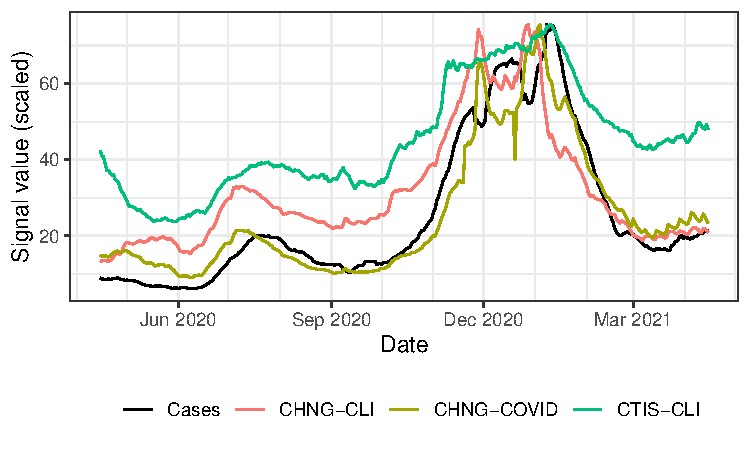
\includegraphics[width=\columnwidth]{fig/time_trends_national.pdf}
\caption{National trends, from April 2020 to April 2021, of four signals in
  the COVIDcast API. The auxiliary signals, based on medical claims data and
  massive surveys, track changes in officially reported cases quite
  well. (They have all been placed on the same scale as reported cases per
  100,000 people.)}
\label{fig:time_trends_national}
\end{figure}

Many of the indicators in the COVIDcast API are intended to track COVID
activity. Five indicators in particular have the closest connections to
confirmed cases:

\begin{itemize}
\item Change Healthcare COVID-like illness (CHNG-CLI): The percentage of
  outpatient visits that are primarily about COVID-related symptoms, based on
  de-identified Change Healthcare claims data.
\item Change Healthcare COVID (CHNG-COVID): The percentage of outpatient visits
  with confirmed COVID-19, based on the same claims data.
\item COVID Trends and Impact Survey CLI (CTIS-CLI): The estimated percentage
  of the population with COVID-like illness based on Delphi's surveys of
  Facebook users.
\item COVID Trends and Impact Survey CLI in the community
  (CTIS-CLI-in-community): The estimated percentage of the population who know 
  someone in their local community that is sick, based the same surveys.
\item Quidel test positivity rate (Quidel-TPR): The percentage of positive
  results among Quidel COVID antigen tests.  
\end{itemize}

Figure~\ref{fig:time_trends_national} compares the first three of these signals
to COVID cases in the United States (from JHU CSSE, smoothed with a 7-day
trailing average) over a year of the pandemic (April 15, 2020 to April 15,
2021), illustrating how they track national trends quite well.  Importantly, 
this same relationship persists across multiple resolutions of the data, down to
smaller geographic regions such as states and counties, as shown in the
supplement.  This will also be illustrated in a more detailed correlation 
analysis in the next subsection.   

% TODO
% RJT: @AR Note what I claimed we would do above!  I'm thinking we can just
% produce a big batch of case trends over the same time period and for the same
% signals, but for each US state (and territory?), and for the 50 most populous
% counties. AND maybe for this (below national) we should use CLI-in-community
% rather than CLI, from the survey

Besides tracking contemporaneous COVID activity, these and other indicators can
be used to improve forecasts of future COVID case trends, as investigated in a
companion paper.

% TODO 
% RJT: @AR Consider for the supplement.  [Or skip it?  Not all that important 
% but I think it would be nice to do.  Maybe you can delegate this to Logan,
% Aaron, Jingjing, etc.] 
% - Hospitalization trends?
% - Hospitalization correlations?
%  (I see you already have a plot for the first ... but I'm a bit bothered by
%  the fact that the HHS data looks to have such strong weekday effects that we
%  don't attempt to correct for ... perhaps we use do a 7-day rolling avg. Made
%  easy with modeltools)
% If we do so, we should refer to it in the text, this subsection (for time
% trends) and next (for correlations)

\subsection{Correlation Analyses}

\begin{figure}[t]
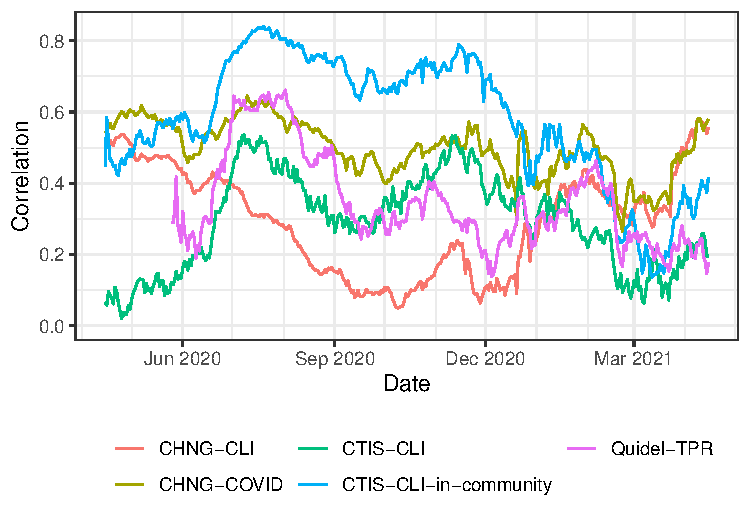
\includegraphics[width=\columnwidth]{fig/geo_wise_corr.pdf}
\caption{Geo-wise correlations with case rates, from April 15, 2020 to April
  15, 2021, calculated over all counties for which all signals were available
  and which had at least 500 cumulative cases by the end of this period.}
\label{fig:geo_wise_correlation}
\end{figure}

To quantify the ability of the signals described above to track trends in COVID
cases, we use the Spearman (rank) correlation and analyze two key correlation
patterns, between each signal and confirmed COVID case rates (cases per 100,000
people):

\begin{enumerate}
\item \textit{Geo-wise correlations} (i.e., on a specific date, do values of the
  signal correlate with case rates across locations?): Formally, let $X_t$ and
  $Y_t$ be vectors of values of a particular signal and case rates, over all
  locations, on date $t$. The geo-wise correlation at time $t$ is defined as
  $\cor(X_t, Y_t)$. This examines whether a signal has the capability to help
  spot locations with high case rates at any given time.

\item \textit{Time-wise correlations} (i.e., at a specific location, do values
  of the signal correlate with case rates across time?): Formally, let $X_\ell$
  and $Y_\ell$ be vectors of a values of a particular signal and case rates,
  over all times, at location $\ell$. The time-wise correlation at time $t$ is
  defined as $\cor(X_\ell, Y_\ell)$. This examines whether changes in a signal
  over time correspond to changes in reported cases at the same location.
\end{enumerate}

Figure~\ref{fig:geo_wise_correlation} shows the geo-wise correlations achieved
by the five signals and COVID case rates (from JHU CSSE, smoothed using a 7-day
trailing average), from April 15, 2020 to April 15, 2021. This calculation is
performed over counties with at least 500 cumulative cases by the end of this
period, and at which all indicators are available (956 counties in total). The
significantly positive correlations suggest that these signals could be useful
in hotspot detection (identifying counties with relatively high COVID activity,
at a given time). Somewhat surprisingly, the survey-based CLI-in-community
signal shows the strongest correlations for much of the time period. This
clearly demonstrates the value of a large-scale survey such as CTIS for tracking
symptoms and case trends, especially when other data is unavailable.

\begin{figure}[t]
  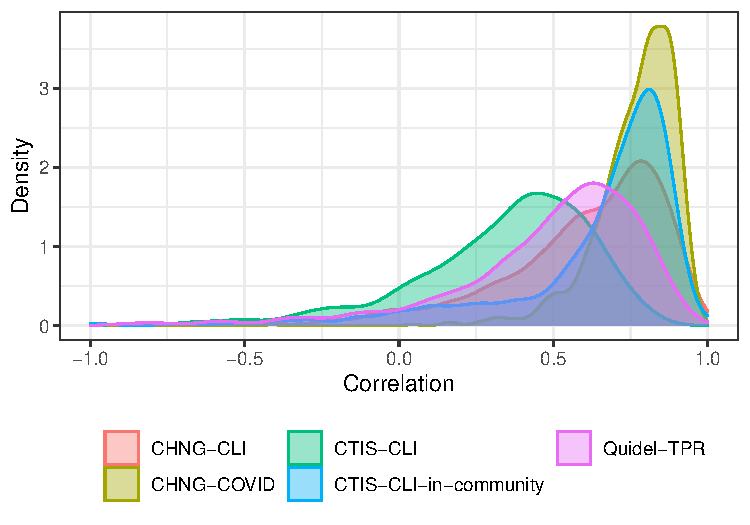
\includegraphics[width=\columnwidth]{fig/time_wise_correlation.pdf}
  \caption{Time-wise correlations with case rates, from April 15, 2020 to April
    15, 2021, calculated over all counties for which all signals were available
    and which had at least 500 cumulative cases by the end of this period.}
  \label{fig:time_wise_correlation}
\end{figure}

Figure~\ref{fig:time_wise_correlation} summarizes time-wise correlations from
these five signals over the same time period, and for the same set of
counties. For each signal, we display the set correlations that it achieves in
histogram form (more precisely, using a kernel density estimate). All signals
produce positive correlations in the majority of counties considered (with very
little mass in each estimated density being to the left of zero). The largest
correlations, in bulk, are achieved by the CHNG-COVID signal; the
CTIS-CLI-in-community is a close second, and the CHNG-CLI signal is third.
There are two noteworthy points:

\begin{itemize}
\item This is different from what is observed in
  Figure~\ref{fig:geo_wise_correlation}, where the CTIS-CLI-in-community signal
  achieves clearly the highest correlations for most of the time
  period. However, it is worth emphasizing that time-wise and geo-wise
  correlations are truly measuring different properties of a signal; and the
  claims signals (CHNG-COVID and CHNG-CLI) seem more appropriate for
  temporal---rather than spatial---comparisons.  We revisit this point in the
  discussion.

\item It is still quite impressive (and surprising) that the
  CTIS-CLI-in-community signal, based on people reporting on the symptoms of
  others around them, can achieve  nearly as strong time-wise correlations to
  confirmed cases as can a signal that is based on picking up the occurrence of
  a confirmed case passing through the outpatient system.
\end{itemize}

\subsection{Helping Robustness}

\begin{figure}[t]
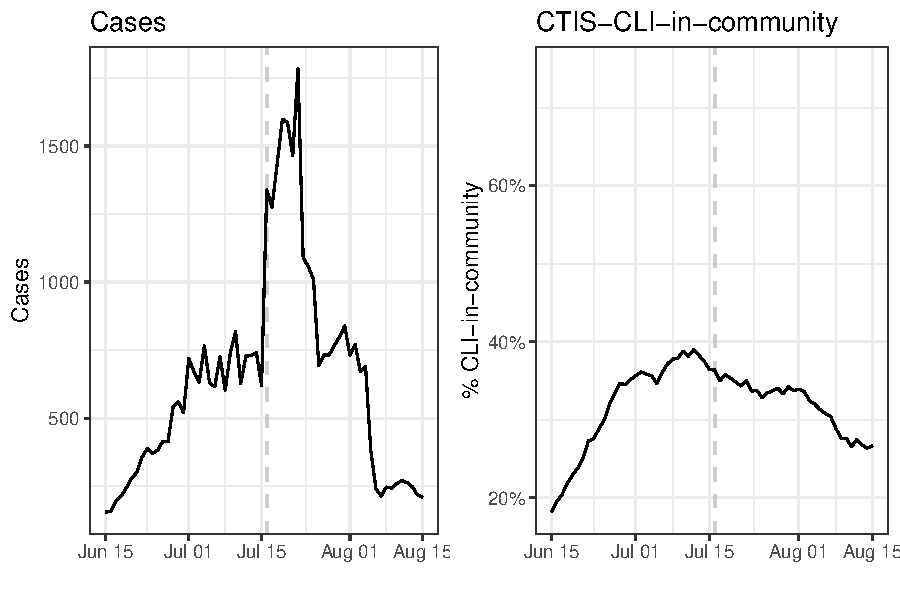
\includegraphics[width=\columnwidth]{fig/bexar_compare.pdf}
\caption{Reported cases per day in Bexar County, Texas during the summer of
  2020. Only July 16, 4,810 backlogged cases were reported, though they
  actually occurred over the preceding two weeks (this shows up as a prolonged
  spike in the left panel due to the 7-day trailing averaging applied to the
  case counts). Daily CTIS estimates of CLI-in-community showed more stable
  underlying trends.}
\label{fig:bexar_compare}
\end{figure}

Public health reporting of COVID tests, cases, deaths, and hospitalizations is
subject to a number of possible delays and problems. For example, COVID testing
data is reported inconsistently by different states using different definitions
and inclusion criteria, and differences in reporting processes mean state data
often does not match data reported to the federal government
\cite{Schechtman:2021}. Case and death data is frequently backlogged and
corrected, resulting in artificial spikes and drops \cite{Simon:2021,
  ArvisaisAnhalt:2021}.

As an example, looking back at Figure \ref{fig:time_trends_national}, we can see
clear dips in the confirmed COVID case curve that occur around the Thanksgiving
and New Year's holidays. This is artificial, and due to the fact that public
health departments usually close over holiday periods, which delays case and
death reporting (for this reason, the artificial dips persist at the state- and
county-level as well). The CLI signal from the survey, on the other hand,
displays no such dips. The claims signals actually display holiday effects going
in the other direction: they exhibit \textit{spikes} around Thanksgiving and New
Year's. This is because they measure the fraction of all outpatient visits with
a certain condition, and the denominator here (total outpatient visits) drops
disproportionately during holiday periods, as people are likely less willing to
go to the doctor for more routine issues. Fortunately, in principle, the holiday
effects in claims signals should be correctable: they are mainly due to
\textit{overall} changes in medical seeking behavior during holiday, periods,
and we can estimate such effects using historical claims data.

As a further example, Figure~\ref{fig:bexar_compare} displays data from Bexar
County, Texas (which contains San Antonio) during July 2020. On July 16, 2020,
4,810 backlogged cases were reported after reporting problems prevented them
from being reported over the past two weeks \cite{Palacios:2021}, resulting in a
clearly visible spike in the left-hand panel of Figure~\ref{fig:bexar_compare}
(case data from JHU CSSE, smoothed using a 7-day trailing average).  Meanwhile,
Delphi's COVID Trends and Impact Survey averaged around 350 responses per day in
Bexar County over the same time period, and was able to estimate the fraction of
the population who know someone in their community with COVID-Like Illness
(CLI). As we can see in the right-hand panel of Figure~\ref{fig:bexar_compare},
this signal was not affected by Bexar County's reporting problems and, as shown
in the last subsection, it is (in general) highly correlated with case rates,
providing an alternate stream of data about COVID activity unaffected by
backlogs. Similar reporting problems have occurred in many jurisdictions across
the United States, making it valuable to cross-check against external sources
not part of the same reporting systems.

\subsection{Revisions Matter}

\begin{figure}[t]
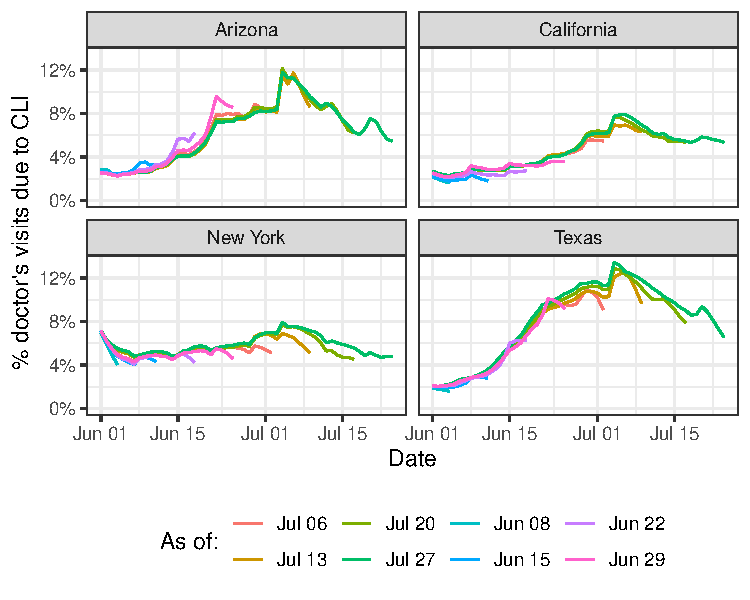
\includegraphics[width=\columnwidth]{fig/dv_as_of.pdf}
\caption{Estimated percentage of doctor's visits due to COVID-like illness
  displayed across multiple issue dates, with later issue dates adding
  additional data and revising past data from prior issue dates.}
\label{fig:dv_as_of}
\end{figure}

The revision tracking feature in the API assists in model-building and
evaluation. Figure~\ref{fig:dv_as_of} illustrates how one COVIDcast medical
claims signal evolved as it was revised across multiple issue dates, in four
different states, between June 1 and August 1, 2020. In each plot, the rightmost
ends of the lines correspond to estimates for the last day that data are
available for each issue date, which are generally the most tentative estimates,
and appear to be significantly biased upward in Arizona in June 2020, and
significantly biased downward in New York throughout June and July 2020.

Claims-based signals typically undergo heavy backfill as additional claims are
processed and errors are corrected; the median relative error between initial
reports and final values is over 20\% for such data, and only after roughly 35
days do estimates typically match finalized values within 5\%. However, the
systematic nature of this backfill, as illustrated in Figure~\ref{fig:dv_as_of},
suggests that statistical models could be fit (potentially separately for each
location) to estimate the final values from preliminary reports. On the other
hand, official public health reporting of COVID cases and deaths can be subject
to revision as death certificates are audited and backlogs cleared, resulting in
thousands of cases and deaths being added or removed. This process is much more
difficult to predict, and thus claims data and other sources may be a useful
stand-in while public health reports are aggregated and corrected.

To reiterate a previous point, when training and validating forecast models (on
historical data), users will want to use data that was known \textit{as of} the
forecast date, not revised versions that only became available much later. The
COVIDcast API makes all historical versions available and easily accessible for
this purpose; and this feature plays a prominent role in our own analysis of
forecasting and hotspot prediction models appearing in a companion paper.

\subsection{New Perspectives}

Auxiliary signals (outside of the standard public health reporting streams) can
serve as indicators of COVID activity, but they can also illuminate other
aspects of the pandemic. To understand the effect of the pandemic on society and
predict its future spread requires a comprehensive view of not just cases and
deaths, but public behavior and beliefs. Measures of mobility reflect social
distancing policies and the potential rate of COVID spread; medical claims data
reflects healthcare-seeking behavior and how it may be affected by local case
rates; measures of COVID vaccine acceptance can guide outreach efforts
\cite{TODO}.

% TODO

% AR: Potentially interesting things to show or comment on:
% - Medical claims data can give info about medical-seeking behavior and how it
% varies with caseload -- e.g. are people deterred from seeking medical care
% because of the high case load?
% - Mobility changes
% - Map of one of the unique signals during an outbreak, e.g. Michigan in April
% 2021

% RJT: @AR Since we already stuff on claims, can we do: mobility, masks, vaccine
% uptake or hesitancy, distancing behaviors, how worried are you?
% How about this (in each case, each point in said plot is a county's signal
% values averaged over some period)
% - Bivariate plot of mask use versus how worried are you
% - Bivariate plot of of how worried are you vs case rates
%- Bivariate plot of of how worried are you vs hospitalizations
% I would be curious to see all three.  And perhaps color code the points by
% region to highlight regional trends

\section{Discussion}

The COVIDcast API provides open access to real-time and geographically-detailed
indicators of COVID activity in the United States that support and enhance
standard public health reporting streams in several ways.

First, several signals in the API closely track COVID activity (over both time
and space); yet they are derived from different data streams (such as surveys,
medical insurance claims, and medical devices), and are therefore not subject to
the same sources of error as public health reporting data. This can be important
both for robustness and situational awareness, allowing decision-makers to
diagnose potential anomalies in standard surveillance streams, and for modeling
tasks such as forecasting and nowcasting. Our companion paper on forecasting
discusses this in more detail.

Second, the API features many other signals that are relevant to understanding
aspects of the pandemic and its effects on the United States population that are
not found in traditional public health streams, such as data on mobility
patterns, Internet search trends, mask wearing, and vaccine hesitancy, to name
just a few. (The latter two are derived from the COVID Trends and Impact Survey;
see our companion paper on this survey for a detailed view of its features and
capabilities.) These signals have already supported pandemic research and
policy-making.

Third, the underlying database tracks all revisions made to the data, allowing
us to query the API to learn ``what was known when'', critical for understanding
the behavior (and potential pitfalls) of real-time surveillance signals. Such
revision data is rarely available in standardized form from other sources.

Finally, we emphasize that unifying many relevant signals into a single common
format, with comprehensive revision tracking, is a valuable goal in and of
itself. No one data source is perfect; each is subject to error. Bringing
numerous signals from different data streams all together, and making access as
convenient as possible for public health researchers, policy makers, modelers,
etc., is a strong testament to our belief that ``the whole is greater than the
sum of its parts''.

There are a number of open questions, and challenges that remain. Each signal is
subject to different biases, such as survey sampling and nonresponse biases or
geographic differences in market share for medical claims data. Claims data can
also be subject to biases during major national holidays and other events that
change health-seeking behavior. Characterizing these biases will be important
for future research using these signals. Several data sources are also subject
to extensive revision and backfill, which must be studied and modeled to enable
real-time use of these sources in forecasting and nowcasting systems. The
breadth and unique features of the COVIDcast API will help facilitate this work,
which will be vital to advancing pandemic modeling and preparedness.

% \matmethods{Please describe your materials and methods here. This can be more than one paragraph, and may contain subsections and equations as required.

% \subsection*{Subsection for Method}
% Example text for subsection.
% }

% \showmatmethods{} % Display the Materials and Methods section

\acknow{Please include your acknowledgments here, set in a single paragraph. Please do not include any acknowledgments in the Supporting Information, or anywhere else in the manuscript.}

\showacknow{} % Display the acknowledgments section

% Bibliography
\bibliography{../../common/covidcast.bib}

\end{document}
